
\documentclass[lang=cn,11pt,a4paper]{elegantpaper}

\title{利用二分法和牛顿公式求解方程的根}
\author{第七小组: 刘阳 \quad 任浩辰 \\ 科目: 数值分析}
\date{\zhtoday}

\begin{document}

\maketitle

\section{实验目的}
通过编程实践,熟练掌握牛顿公式求解方程的根,验证牛顿公式的局部收敛性,比较二分法与牛顿公式的收敛速度,并验证求解结果的正确性。

\section{实验步骤}
\begin{enumerate}
  \item 验证牛顿公式的局部收敛性
  \item 比较二分法与牛顿公式的收敛速度
  \item 验证求解结果的正确性
\end{enumerate}

\section{实验内容}
\subsection{二分法}
  函数$f(x)$在区间$[a,b]$内单调连续,且$f(a)f(b)<0$,根据连续函数的性质可知方程在区间$[a,b]$内一定有唯一的实根。
  通过不断地把函数$f(x)$的零点所在的区间一分为二,使区间的两个端点逐步逼近根,进而得到根的近似值。

\subsection{牛顿公式}
  对于方程
  \begin{equation}
    f(x)=0
  \end{equation}
  
  已知它的近似根$x_k$,则函数$f(x)$在点$x_k$附近可用一阶泰勒展开多项式
  \begin{equation}
    p(x)=f(x_k)+f'(x_k)(x-x_k)
  \end{equation}
  来近似,因此方程$f(x)=0$可近似地表示为$p(x)=0$。后者是个线性方程,求它的根是容易的,我们取 
  $p(x)=0$的根作为$f(x)=0$的新的近似根,记$x_{k+1}$,则有
  \begin{equation}
    x_{k+1}=x_k-\frac{f(x_k)}{f'(x_k)}
  \end{equation}
  这就是牛顿公式。

\section{实验过程及主要代码}
\subsection{验证牛顿公式的局部收敛性}
  因为牛顿法是局部收敛的,收敛性依赖于$x_0$的选取。

  这里我们选取
  \begin{equation}
    f(x)=\frac{5}{6}x^4-4x^3+\frac{23}{6}x^2+3x-\frac{17}{3}
  \end{equation}
  并求$f(x)=0$的根。

  $f(x)$的函数图像为

  \begin{figure}[htbp]
    \centering
    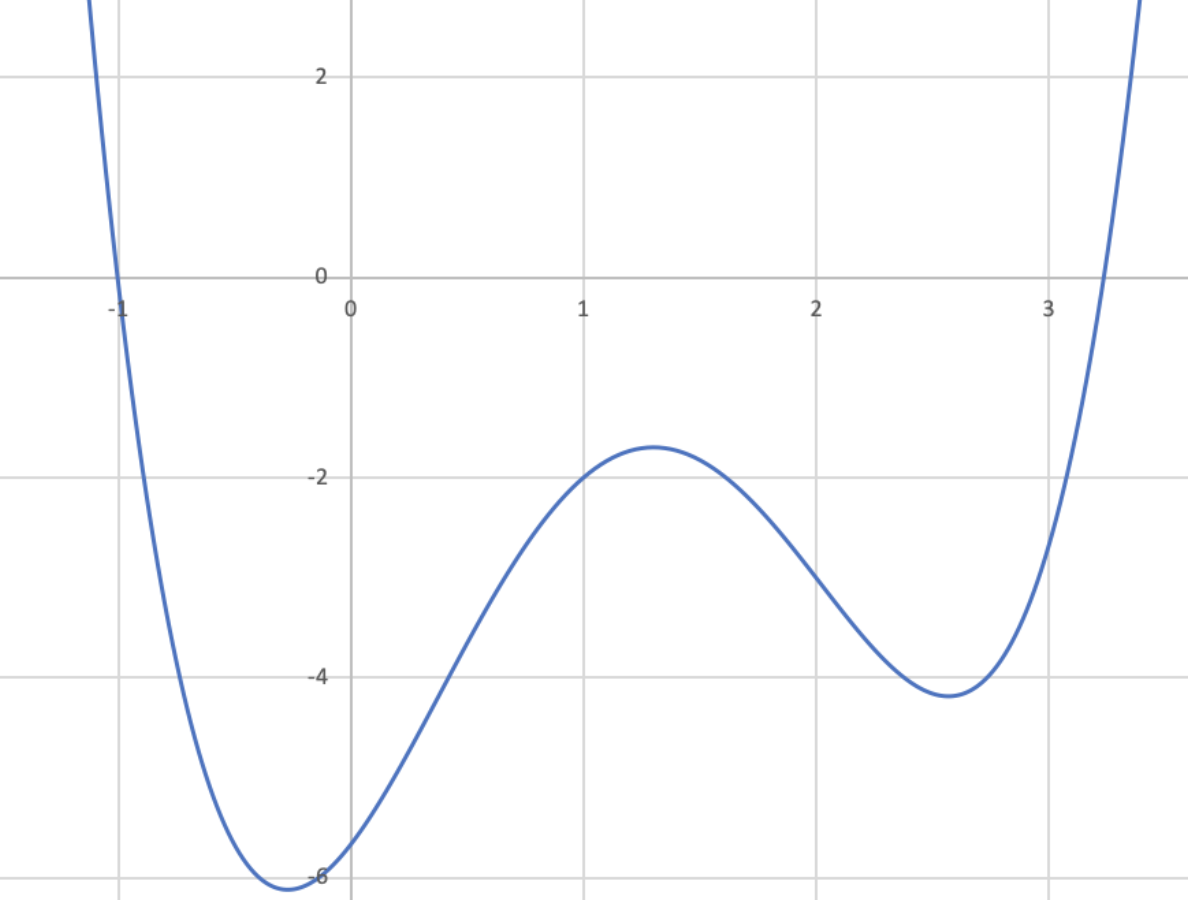
\includegraphics[width=0.5\textwidth]{image/f.png}
  \end{figure}
  
  从图像中我们可以发现,$f(x)=0$存在两个根,两个根分别是$x=-1$和$x=3.2348365$。

  为了验证牛顿公式的局部收敛性,我们分别选择$x_0=3$和$x_0=2$,作为牛顿公式的起始点进行迭代求根(误差不超过$10^{-3}$)。

\subsection{比较二分法与牛顿公式的收敛速度}
  对于上述$f(x)$,分别使用二分法和牛顿公式求解$f(x)=0$的根。

\subsection{验证求解结果的正确性}
  对于上述$f(x)$,使用牛顿公式迭代求解$f(x)=0$的根$x^*$,并带入$f(x)$求函数值,判断$f(x^*)$是否等于或接近$0$。

\subsection{主要代码}
\begin{lstlisting}[language=c++]
  #include <stdio.h>
  #include <cmath>
  
  #define MAX_TIMES 100
  #define e 0.001
  #define ROOT 3.2348365

  /// f(x) = 5/6x^4 - 4x^3 + 23/6x^2 + 3x - 17/3
  double f(double x) {
      return (5.0 / 6.0) * pow(x, 4) - 4 * pow(x, 3)
              + (23.0 / 6.0) * pow(x, 2) + 3 * pow(x, 1) - (17.0 / 3.0);
  }
  
  /// f'(x) = 10/3x^3 - 12x^2 + 23/3x + 3
  double f_d(double x) {
      return (10.0 / 3.0) * pow(x, 3) - 12 * pow(x, 2)
              + (23.0 / 3) * pow(x, 1) + 3;
  }
  
  void Binary() {
      double left = 2.0;
      double right = 4.0;
      double mid;
  
      printf("Binary:\n");
      printf("  k\t xk\n");
      for (int i = 1; i <= MAX_TIMES && (right - left) >= e; i++) {
          mid = (left + right) / 2.0;
          if (f(left) * f(mid) < 0) {
              right = mid;
          } else {
              left = mid;
          }
          printf("%3d  %f\n", i, left);
      }
  }
  
  void Newton() {
  //    double x0 = 2.0;
      double x0 = 3.0;
      double x1;
  
      printf("Newton:\n");
      printf("  k\t xk\n");
      for (int i = 1; i <= MAX_TIMES; i++) {
          x1 = x0 - f(x0) / f_d(x0);
          printf("%3d  %f\n", i, x1);
          if (fabs(x1 -x0) < e) { // 精度达到要求
              break;
          }
          x0 = x1;
      }
      printf("f(%f) = %f\n", x1, f(x1));
  }
  int main() {
      Binary();
      Newton();
  
      return 0;
  }
\end{lstlisting}

\section{实验结果及分析}
\subsection{验证牛顿公式的局部收敛性}
对于$x_0=3$
\begin{figure}[htbp]
  \centering
  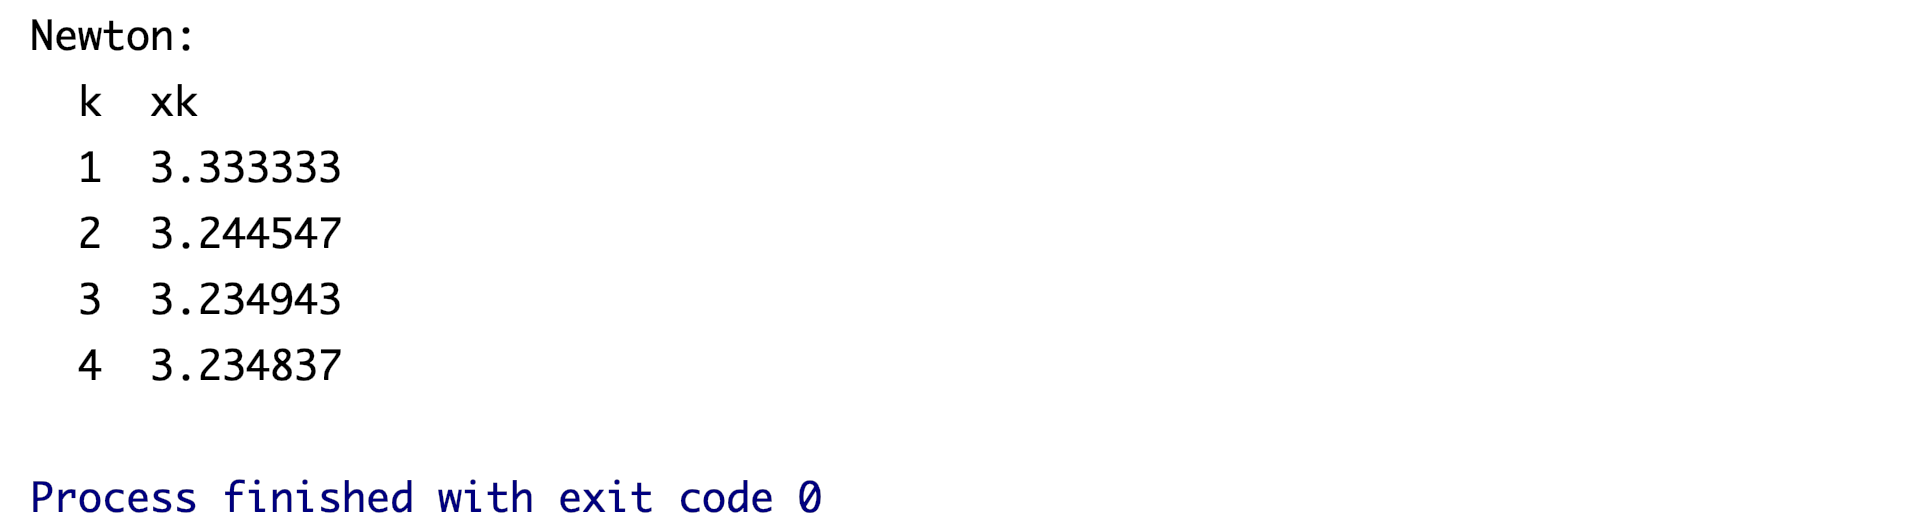
\includegraphics[width=0.85\textwidth]{image/n1.png}
\end{figure}

对于$x_0=2$
\begin{figure}[htbp]
  \centering
  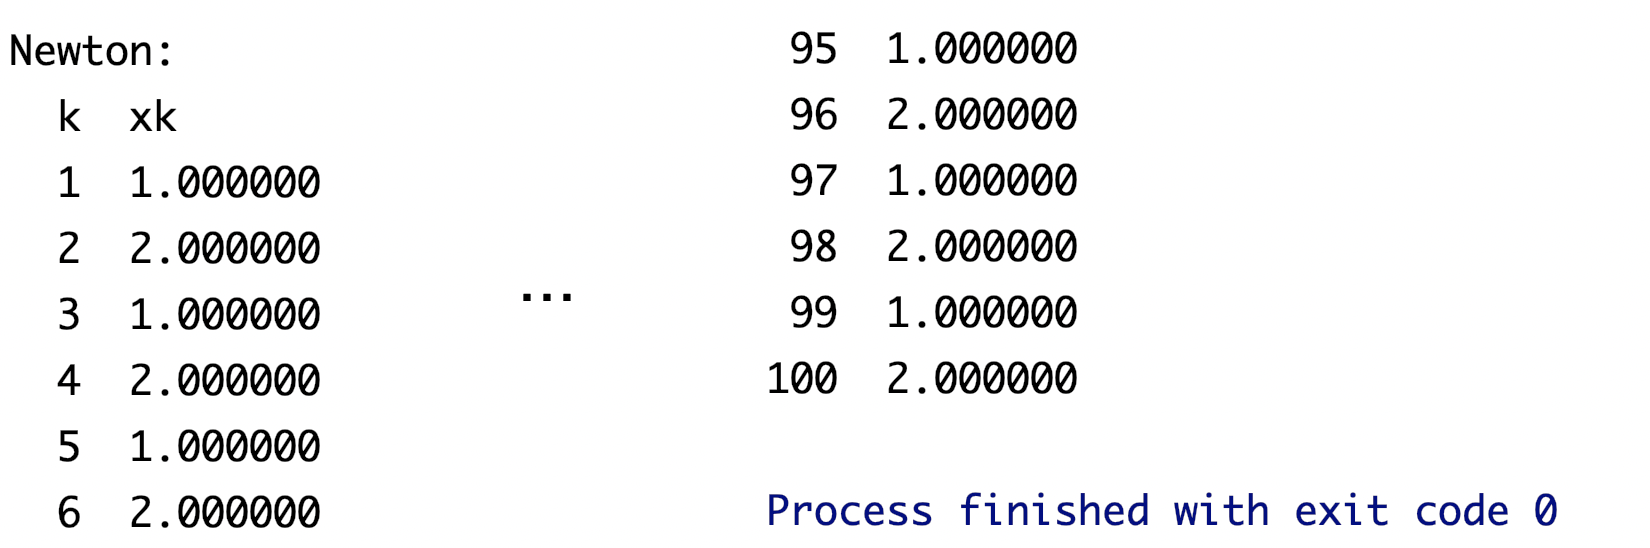
\includegraphics[width=0.8\textwidth]{image/n2.png}
\end{figure}

从$x_0=3$和$x_0=2$的迭代过程,我们可以看出,牛顿公式的收敛性依赖于$x_0$的选取,
$x_0=3$时,通过迭代可以得出$f(x)=0$的近似根为$x=3.234837$,即$x_0=3$收敛,
而$x_0=2$时,$x_k$和$x_{k+1}$在$1$和$2$之间循环,最终超过迭代上限,即$x_0=2$不收敛。

由上可知,牛顿公式具有局部收敛性。

\subsection{比较二分法与牛顿公式的收敛速度}
对于相同的方程$f(x)=0$,使用二分法(选取区间的左端点作为根的近似值)和牛顿法求解根(误差不超过$10^{-3}$),迭代次数以及根输出如下

\clearpage

\begin{figure}[htbp]
  \centering
  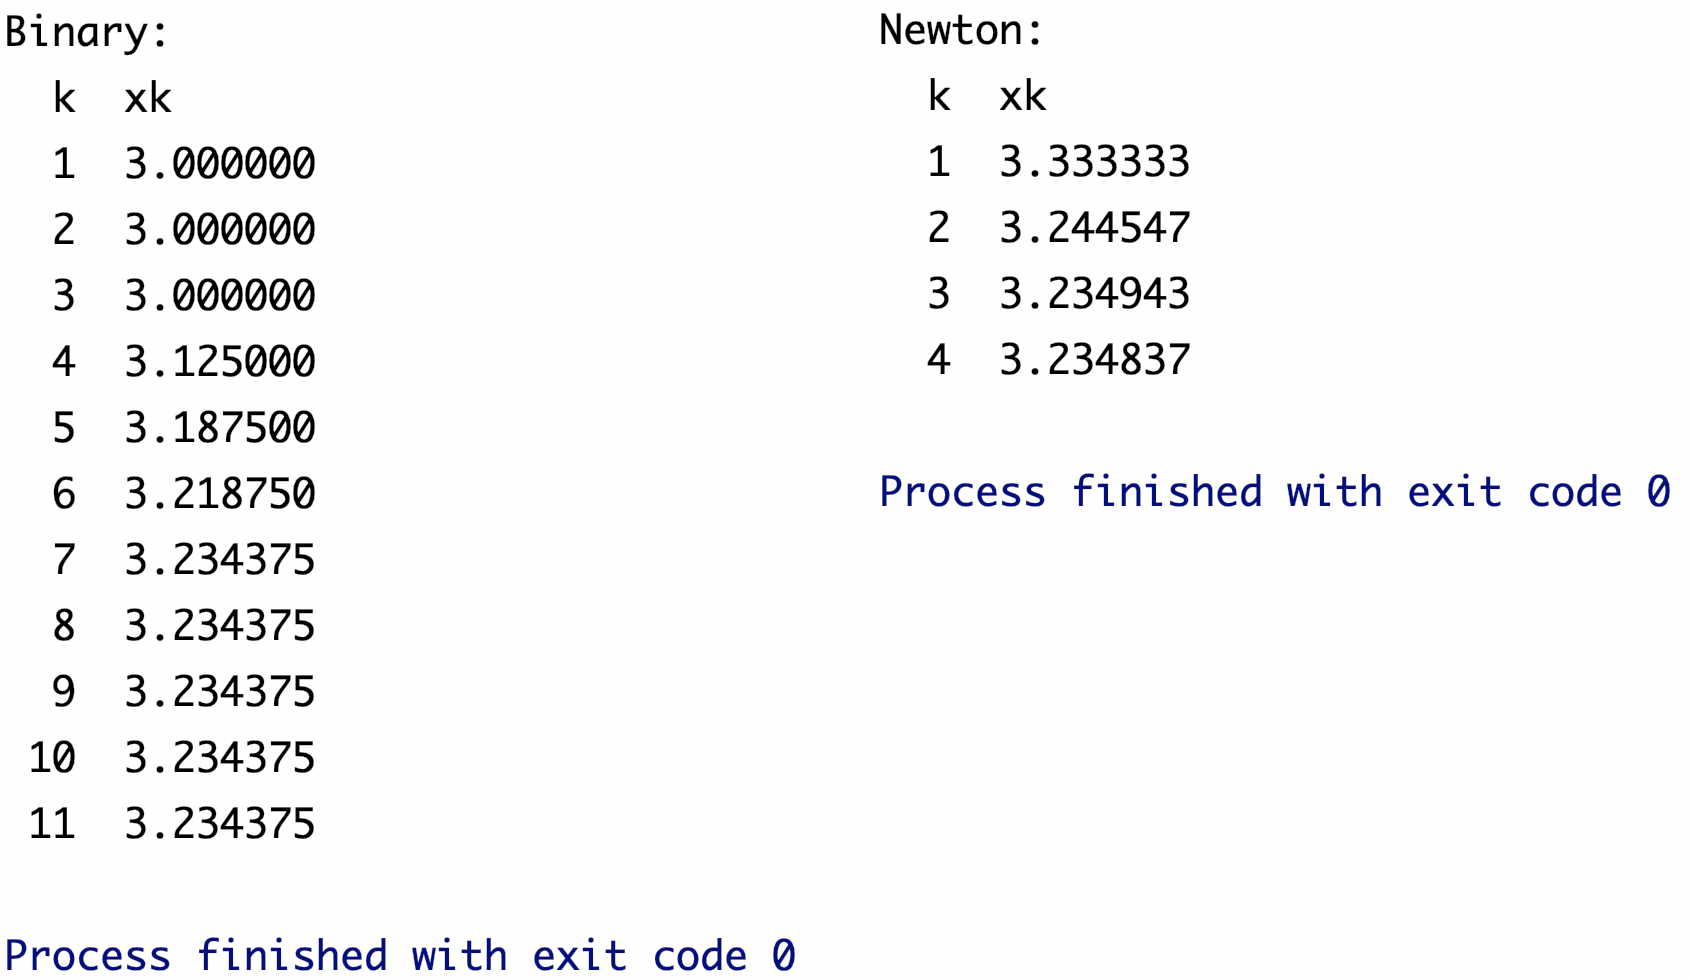
\includegraphics[width=0.8\textwidth]{image/bn.png}
\end{figure}

由此可见,二分法$11$步求得近似根,而牛顿公式仅用$4$步求的近似根,牛顿公式的收敛速度远快于二分法。

\subsection{验证求解结果的正确性}
使用牛顿公式求得的近似根为$x=3.234873$,真实值为$x=3.234836$。

\begin{figure}[htbp]
  \centering
  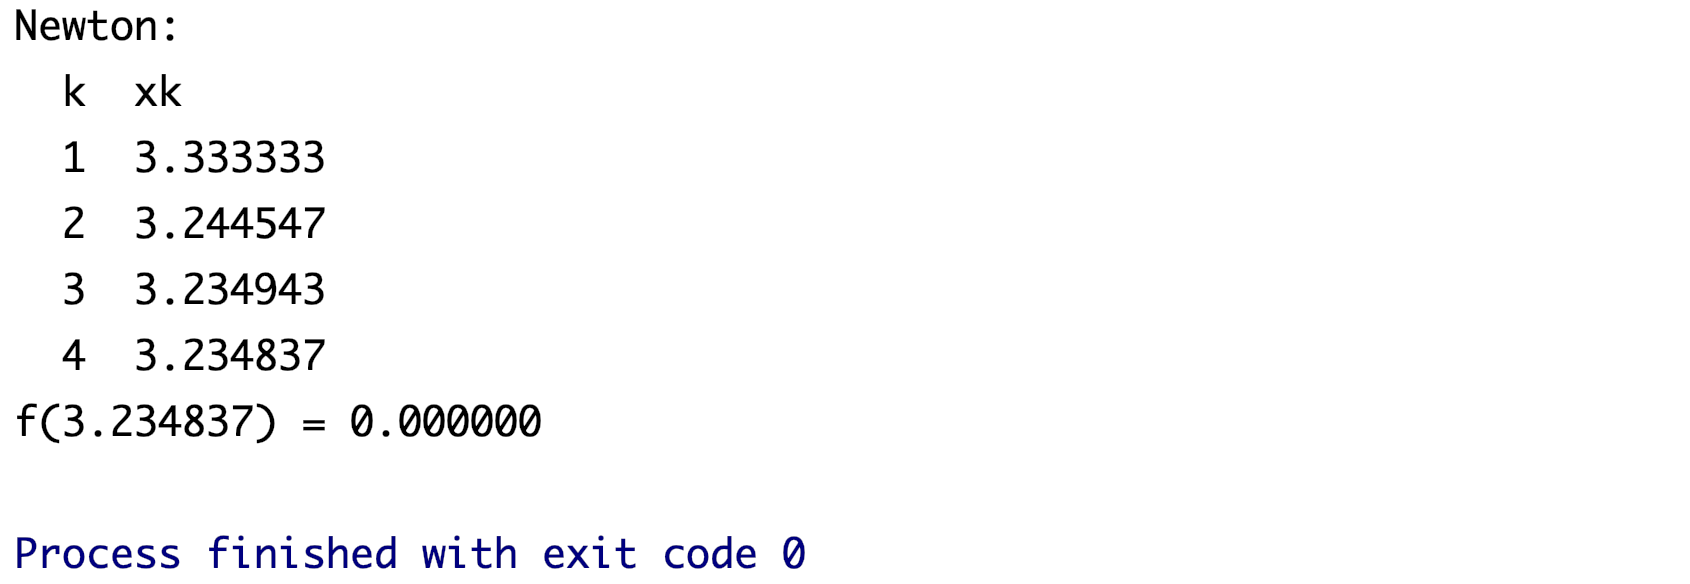
\includegraphics[width=0.8\textwidth]{image/r.png}
\end{figure}

牛顿公式求得的近似根与真实值十分接近,并且近似根的函数值十分接近零,牛顿公式正确。

\section{实验体会}
在这次的实验过程中,使用 C++ 编写了二分法和牛顿公式的相关代码,增强了编程能力,也进一步理解了这两种求近似根的方法。

牛顿公式给了我们一种可以机械化求近似根的方式,不需要我们花费更多时间寻找适合的迭代函数$\varphi(x)$,
并且牛顿公式比二分法有更快的收敛速度,在精度一定的情况下,能更快地求解出近似根,
但是牛顿公式是局部收敛的,也就是说对于某些函数$f(x)$与特定的$x_0$牛顿公式不一定收敛于根$x^*$,
所以在实际使用中可以用其他方法找出处在收敛区域内的$x_0$,再使用牛顿公式求解近似根。

\end{document}
